\documentclass[14pt,a4paper,article]{ncc}
\usepackage[a4paper, mag=1000, left=2.5cm, right=1cm, top=2cm, bottom=2cm, headsep=0.7cm, footskip=1cm]{geometry}
\usepackage[utf8]{inputenc}
\usepackage[T2A]{fontenc}
\usepackage[english,russian]{babel}
\usepackage{indentfirst}
%\usepackage[dvipsnames]{xcolor}
\usepackage{amsfonts} 
\usepackage{amssymb} 
\usepackage{amsmath, etoolbox}
\usepackage{graphicx}
\usepackage{float}
\graphicspath{figure}
\DeclareGraphicsExtensions{.png,.jpg, .jpeg}

%\bibliographystyle{gost-numeric.bbx}
\usepackage{csquotes}
\usepackage[backend=biber]{biblatex}
\addbibresource{literature.bib}

\usepackage{fancyhdr}
\pagestyle{fancy}
\fancyhead[LE,RO]{\thepage}
\fancyfoot{} 

\usepackage{listings}

%\patchcmd\subequations
%{\theparentequation\alph{equation}}
%{\subequationsformat}
%{}{}

%\newcommand{\subequationsformat}{\theparentequation.\arabic{equation}}

\numberwithin{equation}{subsection}


\usepackage[colorlinks]{hyperref}
\hypersetup{linkcolor=black}

\begin{document}

% Title page 
\begin{titlepage}
    \begin{center}
        \textsc{
            Санкт-Петербургский политехнический университет Петра Великого \\[5mm]
            Институт прикладной математики и механики\\[2mm]
            Кафедра прикладной математики
        }   
        \vfill
        \textbf{\large
            Машина опорных векторов\\
            Доклад на тему: \\[3mm]
            ``Асимптотическое поведение LOO-ошибки SVM-классификатора с гауссовым ядром''
            %по курсовой работе \\[3mm]
        }                
    \end{center}

    \vfill
    \hfill
    \begin{minipage}{0.5\textwidth}
        Выполнил: \\[2mm]   
		Студент: Дамаскинский Константин \\
		Группа: 3630102/70201\\
    \end{minipage}


    \vfill
    \begin{center}
        \theyear\ г.
    \end{center}
\end{titlepage}

\tableofcontents
\listoffigures
\listoftables
\newpage

\section{Постановка задачи}

\subsection{Общая формулировка}
Пусть дана тренировочная последовательность $\{x_i, y_i\}, x_i \in \mathbb{R}^n, \; y_i \in \{1, -1\}, \; i \in \overline{1,l}$. Тогда настройка машины опорных векторов состоит в решении следующей задачи оптимизации:

\begin{equation}
\min_{w, b, \xi} \frac{1}{2}w^Tw + C \displaystyle \sum_{i = 1}^{l}\xi_i
\end{equation}
при условии

\begin{align}
y_i(w^T z_i + b) \geq 1 - \xi_i \\
\xi_i \geq 0, i \in \overline{1,l}
\end{align}
где $z_i= \varphi(x_i)$ -- результат отображения тренировочного вектора в пространство размерности $\textrm{dim} w$, $C > 0$ -- штрафной параметр.

К данной задаче квадратичного программирования строится двойственная задача:

\begin{equation}
\min_{\alpha} F(\alpha) = \frac{1}{2}\alpha^TQ\alpha -e^T \alpha
\end{equation}

при условии
\begin{align}
0 \leq \alpha_i \leq C \\
y^T \alpha = 0, i \in \overline{1,l}
\end{align}
где $e=(1, \dots, 1)^T$, $Q$ -- положительно полуопределённая матрица размера $l \times l$, задаваемая по формуле: $Q_{ij}=y_i K(x_i, x_j) y_j; K(x_i, x_j) = \varphi^T(x_i) \varphi(x_j)$ -- \textit{ядро}. Тогда $w= \displaystyle \sum_{i = 1}^{l} \alpha_i y_i \varphi(x_i)$.

В данном докладе мы рассмотрим настройку машины опорных векторов с гауссовым ядром:
\begin{equation}
K(\tilde{x}, \overline{x})= \exp \left( \frac{-\| \tilde{x} - \overline{x} \|^2}{2 \sigma ^2} \right)
\end{equation}

\subsection{LOO-ошибка}

Оценить ошибку обобщения, получаемую при обучении SVM, можно вычислив loo-ошибку (leave-one-out): машину обучают на всей тренировочной последовательности без $i$-го элемента, затем подают на вход $i$-й элемент и проверяют, правильно ли машина его классифицировала. Данную операцию проделывают для всех элементов тренировочной выборки. Доля неверно классифицированных элементов ТП и называется loo-ошибкой.

\section{Построение оптимального SVM-классификатора}

В данном разделе будет показана методика выбора параметров $\sigma$ и $C$, позволяющая построить хорошо обученный SVM-классификатор.

\subsection{Асимптотический анализ поведения SVM}

Будем оценивать поведение машины в крайних возможных значениях штрафного параметра $C \; (C \rightarrow 0, C \rightarrow \infty)$ и параметра рассеяния $\sigma \; (\sigma^2 \rightarrow 0, \sigma^2 \rightarrow \infty)$.

Ниже приведены результаты, полученные в \cite{keerthi}	. Они справедливы при следующих предположениях:

\begin{enumerate}
		\item $l_1> l_2 + 1 > 2$, где $l_i$ -- мощность $i$-ой тренировочной последовательности
		\item $\forall i \neq j: \; x_i \neq x_j$ -- все элементы обучающей выборки различны.
\end{enumerate}

В таком случае имеем следующие \textbf{критерии обучаемости}:
\begin{enumerate}
	\item Сильное недообучение происходит, когда:
	\begin{enumerate}
		\item параметр $\sigma$ конечный и $C \rightarrow 0$
		\item $\sigma \rightarrow 0$ и $C$ -- конечный и достаточно маленький
		\item $\sigma \rightarrow \infty$ и $C$ -- конечный
	\end{enumerate}
	
	\item Сильное переобучение происходит, когда $\sigma \rightarrow 0$ и $C$ очень большой
	\item Если $\sigma$ конечный и $C \rightarrow \infty$, то классификатор хорошо разделяет обучающую выборку на два класса, следовательно, в случае сильно зашумлённой обучающей выборки мы получим переобучение
	\item Если $C = \tilde{C} \sigma^2$ и $\sigma \rightarrow \infty$, где $\tilde{C}=const$, то такой классификатор вырождается в линейный SVM-классификатор с штрафным параметром $C$.
\end{enumerate}

Полученные результаты можно представить графически следующим образом:
 \begin{figure}[H]
	\begin{center}
		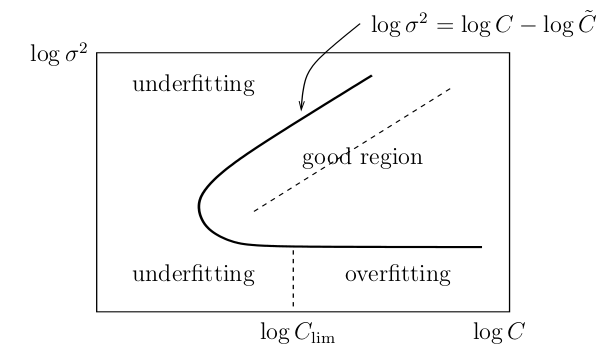
\includegraphics[scale=0.75]{learn_asympt}
		\label{pic:learn_asympt}
		\caption{График обучаемости SVM с гауссовым ядром. По вертикальной оси отложен $\log \sigma^2$, по горизонтальной -- 
		$\log C$}
		\end{center}
	\end{figure}
%\footnote{Вообще говоря, в  \cite{keerthi} loo вводится как \textit{доля} ошибочно классифицированных элементов выборки, однако там же в разделе, посвящённом анализу поведения loo упоминается именно как абсолютное значение неправильно классифицированных элементов ТП.}

\subsection{Комментарии к приведённой иллюстрации}
Underfitting -- область, в которой происходит недообучение модели, overfitting -- переобучение. Любая прямая, описываемая уравнением $\log \sigma^2 = \log C - \log \tilde{C}$, делает классификатор линейным. Пунктирная прямая соответствует выбору $\tilde{C}$, обеспечивающему оптимальную обученность.

Область, отмеченная верхней надписью ``underfitting'', соответствует пункту 1c критериев обучаемости.

Область с напдисью ``good region'' соответствует пункту 4.

Область, отмеченная нижней надписью ``underfitting'', соответствует пунктам 1a и 1b.

Область, отмеченная нижней надписью ``overfitting'', соответствует пункту 2. При этом параметр $C_{lim}$ соответствует значению $C$, левее которого действуют предположения пункта 1b, а правее -- пункта 2.

Горизонтальная прямая, разделяющая ``good region '' и ``overfitting'', соответствует пункту 3.

Стоит отметить, что данный рисунок, как, впрочем, и описание характеристик $C$ и $\sigma$ не являются математически строгими: понятия ``очень большой'' или ``достаточно маленький'' в каждой конкретной ситуации могут означать совершенно разные числовые значения. Однако приведённое графическое разделение пространства гиперпараметров на данные части позволяет получить представление о том, как строить эффективный эвристический алгоритм настройки машины опорных векторов, речь о котором пойдёт в следующем разделе.

\subsection{Подбор $\sigma$ и $C$}

Самым простым методом подбора является метод грубой силы: в логарифмических координатах строится равномерная сетка $r \times r$ и по $\textit{всем узлам}$ ищется комбинация, дающая наименьшую общую ошибку обучения. Однако данный метод, очевидно, является очень непроизводительным, поскольку требует $r^2$ итераций.

Гораздо более рациональный способ подбора оптимальных $\sigma$ и $C$ вытекает из результатов, показанных на рисунке \ref{pic:learn_asympt}: найдём сначала уравнение пунктирной прямой, а затем -- оптимальную комбинацию на ней.

Таким образом, предлагается следующий алгоритм:

\begin{enumerate}
	\item Найдём оптимальный $C$ для \textbf{линейного классификатора} (при $\sigma \rightarrow \infty$) и назовём его $\tilde{C}$
	\item Найдём оптимальную пару, лежащую на прямой, задаваемой уравнением:
	\begin{equation} \label{opt_line}
	\log \sigma^2 = \log C - \log \tilde{C}
	\end{equation}
\end{enumerate}

Поскольку при $\sigma \rightarrow \infty$ SVM с гауссовым ядром ведёт себя как линейный классификатор, подобранный $\tilde{C}$ будет гарантировать хорошую обученность. Во многих задачах распознавания шаблонов линейный классификатор сам по себе даёт удовлетворительный результат.
Поэтому второй шаг можно рассматривать как этап улучшения точности результатов, выдаваемых классификатором.

Рассматривая предложенный двухстадийный подбор параметров на сетке $r \times r$, получим, что процедура поиска в таком случае потребует только $2r$ итераций \footnote{``Двойка'' обусловлена тем, что в уравнении \ref{opt_line} стоит $\log \sigma^2 \equiv 2 \log \sigma$, то есть для перебора на сетке с шагом по $\log C$ равным $r$ понадобится $2r$ операций}, вместо $r^2$ итераций, необходимых для полного перебора всех узлов сетки.

\section{Тестирование эвристического метода настройки SVM-классификатора}

\begin{center}
	\begin{table}[H]
		\resizebox{\textwidth}{!}{
		\begin{tabular}{|c|c|c|c|c|c|}
			\hline
			Название & Число признаков & Мощность ТП & Размерность тестовой выборки & loo. Метод грубой силы & loo. Эвристика \\
			\hline
			banana & 2 & 400 & 4900 & 0.1235 & 0.1178 \\
			\hline
			diabets & 8 & 468 & 300 & 0.2433 & 0.2433 \\
			\hline
			image & 18 & 1300 & 1010 & 0.02475 & 0.02475 \\
			\hline
			splice & 60 & 1000 & 2175 & 0.09701 & 0.10110 \\
			\hline
			ringnorm & 20 & 400 & 7000 & 0.01429 & 0.01800 \\
			\hline
			twonorm & 20 & 400 & 7000 & 0.03100 & 0.02914 \\
			\hline
			tree & 18 & 700 & 11692 & 0.1132 & 0.1246 \\
			\hline
			adult & 123 & 1605 & 29589 & 0.1614 & 0.1614 \\
			\hline
			web & 300 & 2427 & 38994 & 0.02223 & 0.02223 \\
			\hline
		\end{tabular}}
		\caption{Сравнение поведения SVM при двух методах настройки}
	\end{table}
\end{center}

Для настройки SVM методом грубой силы была использована равномерная сетка $[-10; 10] \times [-10; 10]$ с шагом 1 (всего рассматривалась 441 точка пространства гиперпараметров).

При настройке SVM эвристическим методом поиск $\tilde{C}$ осуществлялся путём пятикратной валидации на линейной SVM с использованием равномерной сетки $[-8; 2]$ для $\log C$ и $[-8; 8]$ для $\log \sigma ^ 2$ с шагом 0.5. Всего в совокупности (учитывая поиск $\tilde{C}$) было рассмотрено 54 точки -- в 8 раз меньше, чем в методе грубой силы!

В семи из десяти задач эвристический метод показал loo-ошибку не хуже, чем метод грубой силы. Принимая также во внимание лучшую производительность данного метода по сравнению с методом грубой силы, можно сделать вывод, что данный метод хорошо подходит для применения на практике.

\addcontentsline{toc}{section}{Литература}
\printbibliography

\end{document}
